\documentclass[a4paper, 14pt]{extreport}

\usepackage{vkr}

% Файлы *.bib с информацией об источниках:
\addbibresource{references.bib}


\begin{document}

% Параметры для титульного листа:
\vkrInstitute{Компьютерные науки и прикладная математика}
\vkrDepartment{806}
\vkrProgram{02.04.02 ФИИТ}
\vkrGroup{М8О-213М-21}
\vkrDegree{магистр}

\vkrTitle{Тема выпускной квалификационной работы. Вставьте $\backslash\backslash$ вручную для переноса \\ строки, если тема слишком длинная}

\vkrAuthor{Иван Иванов Иванович}
\vkrSupervisor{Пётр Петров Петрович}
\vkrReviewer{Дмитрий Дмитров Дмитрович}
\vkrHeadOfDepartment{Сергей Сергеев Сергеевич}

\vkrYear{2022}



\vkrAbstract
    
Общий объём работы составляет \ztotpages{} страницы, \totalfigures{} рисунков, \totaltables{} таблиц и ЧИСЛО ИСТОЧНИКОВ использованных источника. \textcolor{red}{Следите здесь за падежами!}

~

СПИСОК КЛЮЧЕВЫХ СЛОВ БОЛЬШИМИ БУКВАМИ

~

Текст реферата.

Что бы воспользоваться шаблоном, и таким образом получить минимальный работающий диплом, скопируйте к себе в папку, или проект в оверлифе, файлы:
\begin{enumerate}
    \item \texttt{mai.png}
    \item \texttt{minimal-example.tex} (можно переименовать)
    \item \texttt{references.bib}
    \item \texttt{vkr.sty}
\end{enumerate}






\vkrIntroduction

Текст введения.





\vkrMain

\section{Литературный обзор}

Текст литературного обзора.

\nocite{duportail:alu}
\nocite{althusser:iia}
\nocite{husserl:pd}
\nocite{husserl:sbe}


\section{Примеры оформления}

\begin{figure}[h]
    \centering
    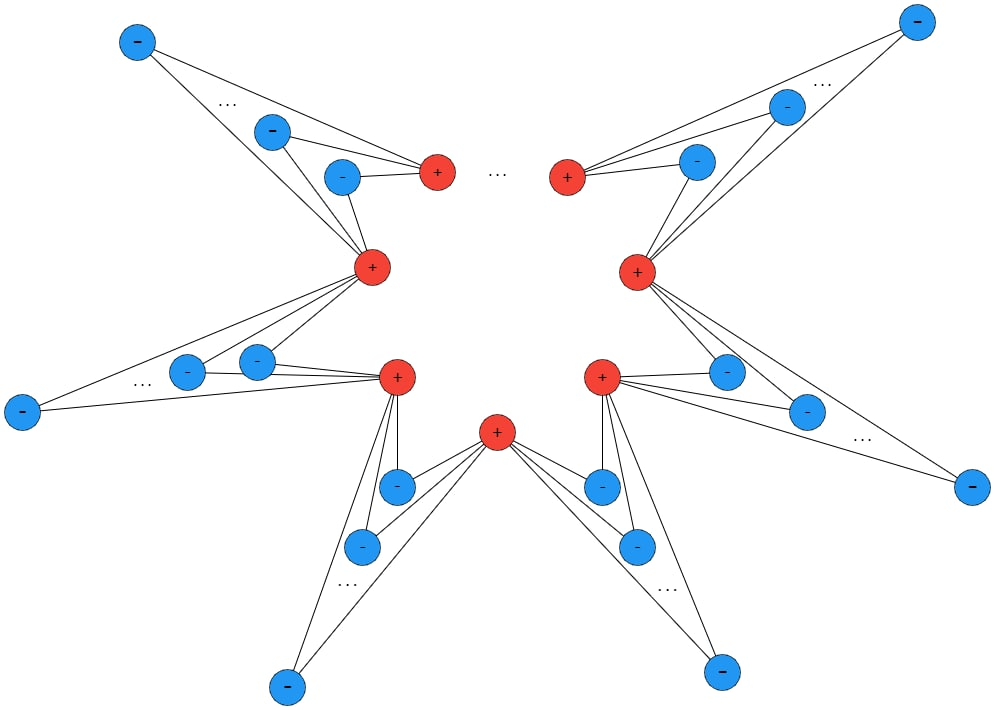
\includegraphics[scale=0.25]{img/graph.jpg}
    \caption{Подпись картинки.}
    \label{fig:example fig 1}
\end{figure}

\begin{table}[h]
    \centering
    \caption{Подпись таблицы.}
    \begin{tabular}{lc|r}
        \textbf{текст} & $1$ & $\alpha$ \\
        \hline
        текст & $1$ & $\beta$ \\
        \textit{текст} & $1$ & $\gamma$ \\
    \end{tabular}
    \label{fig:example table 1}
\end{table}

\begin{equation}
    1 = 2
\end{equation}


\section{Теория}

Текст теоретического обзора.

\subsection{subsection}

\subsubsection{subsubsection}

\paragraph{paragraph}

\section{Реализация}

Текст описания реализации.

\section{Результаты}

Текст результатов.




\section{Практическая часть}

Текст практической части.





\vkrConclution

Текст заключения.




\vkrEnd

\end{document}